\chapter{Rechtlijnige voortplanting van licht}\label{ch:g6:light-propagation}

``\omterm{def:g1:light-and-shadows:source}{Licht} plant zich langs rechte lijnen voort'' heeft je twee jaar
gediend --- bij het verklaren van \omterm{def:g1:light-and-shadows:shadow}{schaduwen}, het richten van
\omterm{def:g5:mirrors-reflection:reflection}{spiegels}, het uitlijnen van drie kaarten en een kaars. Dit jaar
krijgt de oude wet haar officiële naam, haar tekenregels en haar meest
magische gevolg: een camera zonder lens, zonder glas, zonder bewegende
onderdelen --- alleen een gaatje.

\section{De wet, netjes geformuleerd}

\begin{proposition}[Rechtlijnige voortplanting van licht]\label{prop:g6:light-propagation:law}
In heldere \omterm{def:g2:air-around-us:air}{lucht} --- en in elk helder, goed gemengd materiaal zoals
stil water of glas --- plant \omterm{def:g1:light-and-shadows:source}{licht} zich langs rechte lijnen voort. Dat
is de wet van de \emph{rechtlijnige
voortplanting}\index{rechtlijnige voortplanting}: \emph{rechtlijnig}
betekent eenvoudig ``langs rechte lijnen'', en \emph{voortplanting}
noemt het reizen van \omterm{def:g1:light-and-shadows:source}{licht} van plaats naar plaats.
\end{proposition}

\begin{definition}[Straal en bundel]\label{def:g6:light-propagation:ray}
Een \emph{lichtstraal}\index{lichtstraal} is de tekening die de
natuurkundige maakt van één draadje \omterm{def:g1:light-and-shadows:source}{licht}: een rechte lijn met een
pijl voor de looprichting. Echte lampen storten ontelbare draadjes
tegelijk uit: een bundeltje stralen is een \emph{bundel}\index{bundel}.
Drie bundelvormen dekken de praktijk: \emph{divergent} (stralen die
uit één punt uitwaaieren --- elke kleine lamp), \emph{evenwijdig}
(stralen naast elkaar, die elkaar niet naderen en niet verlaten ---
zonlicht, dat zo ver heeft gereisd), en \emph{convergent} (stralen die
naar een punt toe sluiten --- \omterm{def:g1:light-and-shadows:source}{licht} gebundeld door instrumenten die je
over twee jaar leert kennen).
\end{definition}

\begin{omfigure}
\begin{tikzpicture}[scale=0.8]
  \fill[omThm] (0.5,1.3) circle (0.14);
  \foreach \a in {-28,-14,0,14,28} {
    \draw[-Stealth, omThm, thick] (0.6,1.3) -- ++(\a:2.6);
  }
  \node[below, font=\small] at (1.8,-0.1) {divergent};
  \foreach \y in {0.5,1.0,1.5,2.0} {
    \draw[-Stealth, omThm, thick] (4.6,\y) -- (7.4,\y);
  }
  \node[below, font=\small] at (6.0,-0.1) {evenwijdig};
  \foreach \a in {152,166,180,194,208} {
    \draw[-Stealth, omThm, thick] (11.4,1.3) ++(\a:2.6)
      -- ++({\a-180}:2.35);
  }
  \fill[omExo] (11.4,1.3) circle (0.1);
  \node[below, font=\small] at (9.8,-0.1) {convergent};
\end{tikzpicture}

{\small Drie \omterm{def:g6:light-propagation:ray}{bundels}: uitwaaierend vanaf een lamp, evenwijdig
marcherend vanaf de verre Zon, sluitend naar een punt.}
\end{omfigure}

\begin{omfigure}
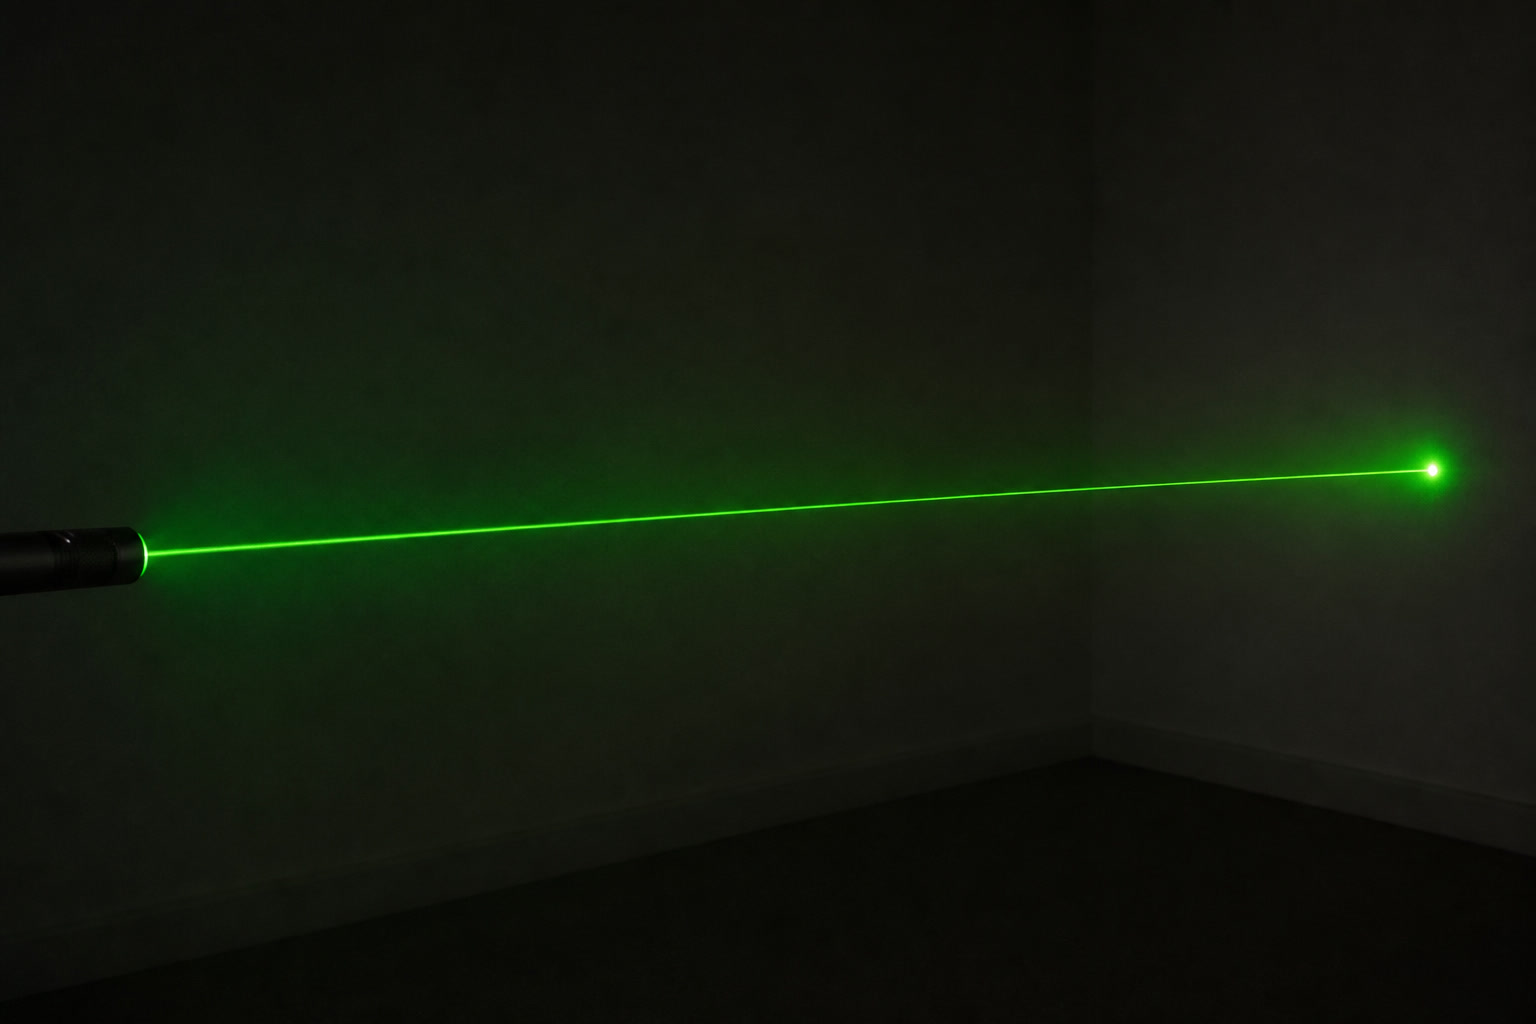
\includegraphics[width=0.55\linewidth]{images/book1/ai/g6-light-laser-fog.jpg}

{\small Een laserbundel zichtbaar gemaakt door mist: één volmaakt rechte lijn van bron tot muur.}
\end{omfigure}

\begin{example}[De wet aan het werk, overal]\label{ex:g6:light-propagation:sightings}
Bouwers kijken langs de rand van een plank om te beoordelen of hij
recht is --- oog, rand en verre uiteinde moeten op één lijn liggen, en
de rechtheid van het \omterm{def:g1:light-and-shadows:source}{licht} is de eed van de rechter. Landmeters zetten
palen op één lijn op het oog; boogschutters en fotografen ``lijnen het
schot uit''; en de driekaartenproef van twee jaar geleden heeft nu een
officiële naam: een toets van de \omterm{prop:g6:light-propagation:law}{rechtlijnige voortplanting}. Elk van
die vakken ruilt een rechte lijn \omterm{def:g1:light-and-shadows:source}{licht} in voor een rechte lijn
materie.
\end{example}

\section{Schaduwen, geconstrueerd}

\begin{method}[Een schaduw met de liniaal construeren]\label{met:g6:light-propagation:shadow}
Voor een kleine lamp $S$, een bal en een scherm erachter:
\begin{enumerate}
  \item teken de straal vanuit $S$ die net langs de bovenrand van de
        bal scheert, en verleng hem recht tot het scherm;
  \item doe hetzelfde met de straal die langs de onderrand scheert
        (en, in drie dimensies, rondom);
  \item tussen de twee scheerpunten op het scherm ligt de
        \emph{schaduw}\index{schaduw}: het gebied dat geen enkele
        rechte straal vanuit $S$ kan bereiken;
  \item de ruimte tussen bal en scherm die door de scherende stralen
        wordt begrensd, is de \emph{schaduwkegel}: een oog daarbinnen
        kan de lamp niet zien.
\end{enumerate}
Nergens gegok: twee liniaallijnen leggen de precieze grootte en plaats
van de \omterm{def:g1:light-and-shadows:shadow}{schaduw} vast.
\end{method}

\begin{omfigure}
\begin{tikzpicture}[scale=0.8]
  \fill[omThm] (0.5,1.9) circle (0.15);
  \node[below, font=\small] at (0.5,1.6) {lamp};
  \draw[thick, fill=omDef, fill opacity=0.3] (4.4,1.9) circle (0.7);
  \draw[very thick] (9.8,-0.6) -- (9.8,4.4);
  \draw[omThm, thick] (0.62,1.99) -- (9.8,3.55);
  \draw[omThm, thick] (0.62,1.81) -- (9.8,0.25);
  \draw[line width=3.5pt, omExo] (9.8,0.25) -- (9.8,3.55);
  \node[right, font=\small] at (9.95,1.9) {schaduw};
  \node[right, font=\small] at (9.95,4.1) {scherm};
  \node[font=\small, omExo] at (7.2,1.9) {schaduwkegel};
\end{tikzpicture}

{\small De \omterm{def:g1:light-and-shadows:shadow}{schaduw}, gebouwd met twee scherende stralen: alles tussen hun
landingspunten ligt buiten het bereik van recht \omterm{def:g1:light-and-shadows:source}{licht}.}
\end{omfigure}

\begin{example}[Groter, kleiner, scherper]\label{ex:g6:light-propagation:sizes}
De constructie voorspelt wat de spelletjes met speelgoed en zaklamp uit
je eerste jaar spelenderwijs vonden: schuif de bal naar de lamp toe en de
scherende stralen waaieren wijder uit --- reuzenschaduw; schuif hem
naar het scherm en ze landen dichter bij elkaar --- \omterm{def:g1:light-and-shadows:shadow}{schaduw} op ware
grootte. En de voorspelling is exact: met de bal halverwege lamp en
scherm spreiden de scherende stralen twee keer de breedte van de bal
--- een \omterm{def:g1:light-and-shadows:shadow}{schaduw} van precies twee keer de grootte van de bal.
Evenredigheid, in \omterm{def:g1:light-and-shadows:source}{licht} getekend.
\end{example}

\section{De camera zonder lens}

\begin{method}[Een gaatjescamera bouwen]\label{met:g6:light-propagation:pinhole}
\begin{enumerate}
  \item neem een doos (een schoenendoos volstaat); maak midden in
        het ene uiteinde een net gaatje ter grootte van een speldenprik;
  \item vervang het tegenoverliggende uiteinde door calqueerpapier
        --- het scherm;
  \item leg een doek over je hoofd en over het schermuiteinde, en
        richt het gaatje op een helder tafereel --- het raam, een
        zonovergoten straat;
  \item kijk naar het calqueerpapier: het tafereel verschijnt, in
        kleur, en beweegt mee met het tafereel ---
        \emph{ondersteboven}.
\end{enumerate}
\end{method}

\begin{proposition}[Waarom het beeld ondersteboven staat]\label{prop:g6:light-propagation:inverted}
De \omterm{prop:g6:light-propagation:law}{rechtlijnige voortplanting} bouwt het \omterm{prop:g5:mirrors-reflection:image}{beeld} en keert het in
dezelfde beweging om. Vanaf de bovenkant van het tafereel reizen de
stralen recht door het gaatje --- en rechte lijnen door een laag
gaatje vanuit een hoog punt moeten \emph{omlaag} verdergaan: de
bovenkant landt onderaan het scherm. Vanaf de onderkant van het
tafereel gaan ze omhoog door het gaatje naar de bovenkant van het
scherm. Elk punt van het tafereel stuurt zijn draadje door die ene
kleine poort, de draadjes kruisen elkaar bij de poort, en het \omterm{prop:g5:mirrors-reflection:image}{beeld}
zet zich omgekeerd in elkaar --- boven voor onder, links voor rechts.
\end{proposition}

\begin{omfigure}
\begin{tikzpicture}[scale=0.8]
  \draw[-Stealth, very thick, omDef] (0.7,0.6) -- (0.7,3.2);
  \node[left, font=\small] at (0.55,1.9) {het tafereel};
  \draw[thick] (5.6,-0.2) -- (5.6,1.55) (5.6,2.05) -- (5.6,3.8);
  \node[above, font=\small] at (5.6,3.85) {wand met gaatje};
  \draw[omThm, thick] (0.7,3.2) -- (5.6,1.8) -- (10.4,0.42);
  \draw[omThm, thick] (0.7,0.6) -- (5.6,1.8) -- (10.4,2.85);
  \draw[very thick] (10.4,-0.2) -- (10.4,3.8);
  \draw[-Stealth, very thick, omDef] (10.4,2.85) -- (10.4,0.42);
  \node[right, font=\small] at (10.55,1.6)
    {het beeld: ondersteboven};
\end{tikzpicture}

{\small De gaatjescamera: elk draadje \omterm{def:g1:light-and-shadows:source}{licht} loopt recht door de kleine
poort, de draadjes kruisen elkaar, en het tafereel landt omgekeerd op
het scherm.}
\end{omfigure}

\begin{remark}[Een oude en eerbiedwaardige doos]\label{rem:g6:light-propagation:history}
De gaatjeskamer --- \emph{camera obscura}, ``donkere kamer'' --- is
eeuwen ouder dan de fotografie: sterrenkundigen bekeken
zonsverduisteringen veilig op haar scherm, en schilders trokken haar
\omterm{prop:g5:mirrors-reflection:image}{beelden} over om het perspectief kloppend te krijgen. Elke moderne
camera, en je eigen oog, houdt haar bouwwijze aan: een kleine poort
voor het \omterm{def:g1:light-and-shadows:source}{licht}, een scherm voor het \omterm{prop:g5:mirrors-reflection:image}{beeld} --- en ja, het
\omterm{prop:g5:mirrors-reflection:image}{beeld} achter in je oog staat ook ondersteboven; je hersenen draaien
het beleefd om. Eén wet van de rechte lijn, geduldig gevolgd,
verklaart de familiecamera en de halve geschiedenis van het
beeldmaken.
\end{remark}

\section{Oefeningen}

\begin{exercise}[$\star$]\label{exo:g6:light-propagation:1}
Zeg de wet van de \omterm{prop:g6:light-propagation:law}{rechtlijnige voortplanting} in je eigen woorden, en
pak allebei de lange woorden uit.
\end{exercise}

\begin{exercise}[$\star$]\label{exo:g6:light-propagation:2}
Noem de drie bundelvormen, elk met één echte bron of situatie. In
welke vorm komt zonlicht aan, en waarom?
\end{exercise}

\begin{exercise}[$\star$]\label{exo:g6:light-propagation:3}
Een bouwer kijkt langs de rand van een plank om te controleren of hij
recht is. Wat speelt in die toets de liniaal? Welke wet wordt
vertrouwd?
\end{exercise}

\begin{exercise}[$\star$]\label{exo:g6:light-propagation:4}
Wat bepaalt bij de schaduwconstructie de rand van de \omterm{def:g1:light-and-shadows:shadow}{schaduw} op het
scherm? Wat geldt er voor een oog dat in de schaduwkegel staat?
\end{exercise}

\begin{exercise}[$\star$]\label{exo:g6:light-propagation:5}
Met \cref{ex:g6:light-propagation:sizes}: de bal staat halverwege lamp
en scherm. De bal is \qty{6}{cm} breed --- hoe breed is zijn
\omterm{def:g1:light-and-shadows:shadow}{schaduw}? En als de bal dicht bij het scherm komt?
\end{exercise}

\begin{exercise}[$\star$]\label{exo:g6:light-propagation:6}
Waar landt in de gaatjescamera het \omterm{def:g1:light-and-shadows:source}{licht} van de bovenkant van het
tafereel op het scherm? Geef de reden in één zin.
\end{exercise}

\begin{exercise}[$\star$]\label{exo:g6:light-propagation:7}
Een vriend zwaait met zijn rechterhand voor je gaatjescamera. Welke
kant zwaait er op het scherm, en welke kant staat boven? (Pas op ---
twee omkeringen.)
\end{exercise}

\begin{exercise}[$\star$]\label{exo:g6:light-propagation:8}
Noem twee historische of moderne gebruikers van de camera obscura, en
het werk dat ze voor elk deed.
\end{exercise}

\begin{exercise}[$\star\star$]\label{exo:g6:light-propagation:9}
Construeer (schets met een liniaal): lamp links, een muntvormige
blokkeerder, scherm rechts --- en zet de \emph{lamp} dan twee keer zo
ver van de munt, met het scherm op zijn plaats. Wat gebeurt er volgens
je eigen tekening met de grootte van de \omterm{def:g1:light-and-shadows:shadow}{schaduw}? Breng dat in
overeenstemming met de waaier van scherende stralen.
\end{exercise}

\begin{exercise}[$\star\star$]\label{exo:g6:light-propagation:10}
Op een zonnige dag zijn boomschaduwen scherp; onder een bewolkte hemel
verdwijnen \omterm{def:g1:light-and-shadows:shadow}{schaduwen} bijna. Verklaar beide hemels met stralen en
bronnen --- wat voor ``lamp'' is een heel grijs wolkendek?
\end{exercise}

\begin{exercise}[$\star\star$]\label{exo:g6:light-propagation:11}
Het \omterm{prop:g5:mirrors-reflection:image}{beeld} van de gaatjescamera wordt helderder als het gaatje groter
wordt --- maar het wordt onscherp. Verklaar beide effecten met
draadjes door de poort: wat laat een wijde poort elk punt van het
tafereel op het scherm schilderen?
\end{exercise}

\begin{exercise}[$\star\star\star$]\label{exo:g6:light-propagation:12}
Onder een lommerrijke boom vult de grond zich tijdens een gedeeltelijke
zonsverduistering met honderden sikkeltjes. Zet de verklaring in
elkaar met dit hoofdstuk: wat zijn de gaatjes tussen de bladeren, wat
is op een gewone dag elke lichte vlek, en waarom worden de vlekken
sikkelvormig zodra de Zon dat wordt? (Het hoofdstuk over
zonsverduisteringen van volgend jaar zal trots op je zijn.)
\end{exercise}

\section{Probleem: het schaduwtheater}

\begin{problem}[{Weekendprobleem --- het schaduwtheater van het gezin;
poppen op maat gebracht met evenredigheid, een gaatjesfinale; de rechte
lijnen van het licht runnen de voorstelling}]\label{pb:g6:light-propagation:1}
Een laken als scherm, één kleine felle lamp, kartonnen poppen: zaterdag
is de première, en de toneelploeg werkt met linialen.

\medskip\noindent\textbf{Deel I --- Het toneel opbouwen.}
De lamp staat \qty{4}{m} van het scherm.
\begin{enumerate}
  \item Een pop die tegen het scherm wordt gehouden werpt een
        \omterm{def:g1:light-and-shadows:shadow}{schaduw} van precies haar eigen grootte. Waarom?
  \item De drakenpop is \qty{20}{cm} hoog. Halverwege gehouden ---
        \qty{2}{m} van lamp en scherm --- hoe hoog is haar
        \omterm{def:g1:light-and-shadows:shadow}{schaduw}?
  \item Voor de finale moet de draak \qty{80}{cm} hoog uittorenen. De
        ploeg schuift hem naar de lamp toe: op $1$ \omterm{def:g2:measuring-length:units}{meter} van de lamp
        spreiden de scherende stralen vier keer de grootte van de
        pop. Controleer: klopt \qty{80}{cm}, en op welk deel van de
        afstand lamp--scherm staat de pop?
  \item Waarom moet de lamp van het theater klein en bloot zijn, en
        geen brede matglazen bol? (Wat zou de bol met de scherpe
        randen van de draak doen?)
\end{enumerate}

\medskip\noindent\textbf{Deel II --- Toneeltechniek met stralen.}
\begin{enumerate}[resume]
  \item De wolvenpop moet tijdens haar scène dreigend groeien zonder
        dat de arm van de poppenspeler in \omterm{prop:g5:mirrors-reflection:image}{beeld} komt. Welke kant op
        wordt de pop bewogen, en wat gebeurt er met de randen van
        haar \omterm{def:g1:light-and-shadows:shadow}{schaduw} terwijl ze groeit? (De randen worden iets
        zachter --- aanvaard dat en verklaar het met de kleine maar
        niet puntvormige lamp.)
  \item Twee poppen op dezelfde afstand mogen elkaar niet
        beschaduwen. Wat moet er waar zijn over de rechte lijnen van
        de lamp door elke pop?
  \item Een hand glijdt op een derde van de weg vanaf de lamp tussen
        lamp en draak. Wiens \omterm{def:g1:light-and-shadows:shadow}{schaduw} is groter op het scherm, die van
        de hand of die van de draak, en waarom?
  \item De schurk moet ogenblikkelijk verdwijnen. Geef met stralen in
        de hand twee manieren: één door de pop te bewegen, één met
        een tweede, dichterbij staande blokkeerder.
\end{enumerate}

\medskip\noindent\textbf{Deel III --- De gaatjesfinale.}
Voor de laatste scène maakt de ploeg van het theater zelf een camera
obscura: straatlantaarn buiten, gaatje in het luik, schermlaken door
de kamer.
\begin{enumerate}[resume]
  \item De straatlantaarn hangt buiten hoog. Waar landt haar
        \omterm{prop:g5:mirrors-reflection:image}{beeld} op het laken --- hoog of laag? Waarom?
  \item Een late fietser rijdt van links naar rechts voorbij. Welke
        kant op glijdt het \omterm{prop:g5:mirrors-reflection:image}{beeld} van de fietser over het laken?
  \item Het publiek wil een helderder \omterm{prop:g5:mirrors-reflection:image}{beeld}, dus vergroot de ploeg
        het gaatje tot een opening ter grootte van een munt. Wat
        wordt er van de voorstelling, en waarom?
  \item Slotzin van het programmaboekje: noem in één zin de ene wet
        die de hele avond heeft gerund --- beide theaters, alle
        \omterm{def:g1:light-and-shadows:shadow}{schaduwen}, en de omgekeerde straat.
\end{enumerate}
\end{problem}
